\documentclass[12pt]{report}

\usepackage[english]{babel}
\usepackage[utf8x]{inputenc}
\usepackage{amsmath}
\usepackage{graphicx}
\usepackage{multirow}
\usepackage[hypcap]{caption}
\usepackage{setspace} 

\title{Lab 3: Stall}
\author{Zachary Tschirhart \\
	\small \\
	\small Department of Aerospace Engineering and Engineering Mechanics \\
	\small \textbf{ASE 167M (Wed 3:00-4:00)} \\
	\small Lab Partners: Zachary May, Joshua Eboh, and Brian Huber \\
	\small
	\small TA: Noble Hatten}

\date{February 20, 2013}


\begin{document}
\maketitle

\begin{abstract}
In this lab, the simulator allowed replication of a stall by slowly reducing the power control whilst maintaining level flight. In order to maintain level flight, an increase of the angle of attack was required. This simulation was performed on the GAT-1 flight simulator and was used to show the effects of gross weight, flaps, and landing gear on the stall speed of an aircraft. Additionally, students were able to feel the effects of the stall and learned how to maneuver out of a stall situation. Through various tests, it was verified that a stall is caused by the slowing of flow over an aircraft wing to a point where the pilot cannot compensate for lack of lift by further increasing the angle of attack. Increasing the flaps did allow the aircraft to fly in a reduced stall speed. It was also confirmed that landing gear had no effect on stall speed, while the reduction in weight had a large impact on an increased stall speed. 
\end{abstract}


\tableofcontents
\pagebreak

\setcounter{secnumdepth}{0}





\section{Objectives}
\doublespacing
The three main objectives that should be achieved upon completion of this lab are to explain the cause of aircraft stall and understand how it is caused, measure the effects of flap settings and landing gear position on the stall speed of an aircraft, and, lastly, verify the effects of gross weight on the stall speed of an aircraft.





\section{Procedure}

\begin{itemize}
\item Perform pre-flight checklist as given in the flight manual
\item Set gross weight to 1100 lbs.
\item Use checklist given on the Flight Package for takeoff and climb. Retract landing gear at 50 ft.
\item Climb to 3500 ft., and level off.
\item Perform stall with gear up and no flaps. Maintain level flight by pulling back on the control yoke for each stall and record the stall speed.
\item Perform stall with gear down and no flaps. 
\item Perform stall with gear up and Half flaps. 
\item Perform stall with gear down and Half flaps.
\item Perform stall with gear up and Full flaps. 
\item Perform stall with gear down and Full flaps.
\item Set gross weight to 2100 lbs.
\item Perform stall with gear up and no flaps. 
\item Perform stall with gear down and no flaps. 
\item Perform stall with gear up and Half flaps. 
\item Perform stall with gear down and Half flaps.
\item Perform stall with gear up and Full flaps. 
\item Perform stall with gear down and Full flaps.
\item Establish normal glide to land (idle power).
\item Descend, Land, and perform shutdown checklist as given in the flight manual.
\end{itemize}





\section{Discussion}
\doublespacing
The force created by an aircraft wing is caused by a difference in pressure over a planform area, resulting in a force along the body y-axis and perpendicular to the velocity vector. This force is usually referred to as lift, which is described as,
\begin{equation}
	L = \frac{1}{2} \rho V^{2} C_{L} S
	\label{equation:equation1}
\end{equation}
Where S is the area of the airfoil on the aircraft, \(\rho\) is the density of air which varies based on altitude, \(C_{L}\) is the coefficient of lift that is a function of area of attack and the shape of the airfoil, and V represents the velocity at which the airflow is traveling over the airfoil. The angle of attack, \(\alpha\) ,is defined as the angle between the relative wind axes and the chord line of the wing, as seen in Figure \ref{fig:Figure1}. When the aircraft is in steady and level flight, the lift is equal to the weight of the plane which is an assumption easily made. This can be represented as,\\
\begin{equation}
	W = \frac{1}{2} \rho V^{2} C_{L} S
	\label{equation:equation2}
\end{equation}
In order to solve for the speed at which the aircraft will stall, the velocity will need to be at the minimum while the coefficient of lift will need to be at it's maximum, which, in this lab, is achieved by changing the angle of attack. The equation below solves for the stall speed,
\begin{equation}
	V_{Min Stall} = \sqrt{\frac{2W}{\rho S C_{L max}}}
	\label{equation:equation3}
\end{equation}
Since density and airfoil area were not being tested (constant altitude and constant wing area), the only variation that occurred were weight and the coefficient of lift, which are inversely related. Thus, in order to decrease the stall velocity, one must either decrease weight or increase the coefficient of lift. Since we are assuming the coefficient of lift is at it's maximum for a certain set of parameters, the flaps engaged and angle of attack increased, the only real factor is the weight of the aircraft. In order to predict the stall speed of an aircraft, a simple ratio can be applied in finding the new stall speed given a previous stall speed and weight, along with the intended stall speed. The equation and simplification can be seen below,
\begin{equation}
   \frac{V_{Min Stall 2}}{V_{Min Stall 1}} = \frac{\sqrt{\frac{2 W_{2}}{\rho S C_{L max}}}}
												  {\sqrt{\frac{2W_{1}}{\rho S C_{L max}}}}
										   = \sqrt{\frac{W_{2}}{W_{1}}}
   \label{equation:equation4}
\end{equation}
Solving for \(V_{Min Stall 2}\) produces,
\begin{equation}
	V_{Min Stall 2} = V_{Min Stall 1} \sqrt{\frac{W_{2}}{W_{1}}}
	\label{equation:equation5}
\end{equation}
The relative error between the recorded and the model stall speeds, was calculated with the equation, 
\begin{equation}
	error = \frac{V_{recorded} - V_{model}}{V_{model}} * 100
	\label{equation:equation6}
\end{equation}
Where \(V_{recorded}\) is the speed at which was recorded during the experiment and \(V_{model}\) was the speed calculated from the given values in Figure\ref{fig:Figure2}





\section{Results}
\doublespacing
The experiment had clear implications as to why the stall speeds changed with respect to deployment of flaps and increasing the angle of attack. As seen in Table\ref{tab:Table1}, the stall speed decreased as the flaps were deployed to the half position and even more so in the full position. This trend is observed in both weight classes. The stall speed between the two aircraft weights is also clear, as the heavier aircraft has a consistently higher stall speed across all flap and gear settings than the lighter configuration. As with the gear configuration, Table\ref{tab:Table1} clearly shows that it has very little effect on stall speed. 

It can be seen that the model predicted values in Table\ref{tab:Table2} are closely related to the actual results recorded with little variation. This verification shows that the Equation 5 holds as a relatively good prediction on what the stall speed will be, given a few parameters.





\section{Conclusion}
\doublespacing
Once the lab was complete and the the results verified, it was easy to determine that the cause of a stall of an aircraft is when the airspeed for a particular gross weight and coefficient of lift is too low to create the lift needed to counter the aircraft's weight. This is apparent since an aircraft in steady flight only needs to have a lift force of the same magnitude as the weight. It was confirmed that the angle of attack increased the coefficient of lift of the aircraft until a critical angle was reached where a sudden decrease of lift occurs, thus creating a stall. The gross weight had a large effect on the minimum speed the aircraft could fly at without stalling.





\section{Recommendations}
\doublespacing
The experiment could be improved by testing more conditions, including more gross weights of the aircraft, in order to get a better sense of where the stall speeds of the aircraft are.

\begin{thebibliography}{0}
\bibitem{notes} Eduardo Gilden, Greg Holt, Kyle DeMars, George Jacobellis {\em ASE 167M Flight Dynamics Laboratory Flight Simulator Experiments and Computer Projects. s.l. : The University of Texas at Austin Department of Aerospace Engineering}  2012.
\end{thebibliography}
\addcontentsline{toc}{section}{Bibliography}





\section{Appendix}

\begin{table}[h]
\centering
\begin{tabular}{|l|l|l|l|l|l|l|} \hline
	\multicolumn{7}{|c|}{Airspeed (MPH)} \\ \hline
	\multicolumn{1}{|c|}{} & 
		\multicolumn{3}{|c|}{1100 lbs} & 
		\multicolumn{3}{|c|}{2100 lbs} \\ \hline
	\multicolumn{1}{|c|}{} &
		\multicolumn{1}{|c|}{0 flaps} &
		\multicolumn{1}{|c|}{1/2 flaps} &
		\multicolumn{1}{|c|}{Full flaps} &
		\multicolumn{1}{|c|}{0 flaps} &
		\multicolumn{1}{|c|}{1/2 flaps} &
		\multicolumn{1}{|c|}{Full flaps} \\ \hline
	\multirow{1}{*}{Gear up} & 45 & 42 & 39 & 62 & 56 & 51\\ \hline
	\multirow{1}{*}{Gear down} & 45 & 42 & 40 & 62 & 56 & 52\\ \hline
\end{tabular} \\
\caption{Experimental results for a CESSNA 150} \label{tab:Table1}
\end{table}


\begin{table}[h]
\centering
\begin{tabular}{|l|l|l|l|l|l|l|} \hline
	\multicolumn{7}{|c|}{Airspeed (MPH) and Relative Error (\%)} \\ \hline
	\multicolumn{1}{|c|}{} & 
		\multicolumn{3}{|c|}{1100 lbs} & 
		\multicolumn{3}{|c|}{2100 lbs} \\ \hline
	\multicolumn{1}{|c|}{} &
		\multicolumn{1}{|c|}{0 flaps} &
		\multicolumn{1}{|c|}{1/2 flaps} &
		\multicolumn{1}{|c|}{Full flaps} &
		\multicolumn{1}{|c|}{0 flaps} &
		\multicolumn{1}{|c|}{1/2 flaps} &
		\multicolumn{1}{|c|}{Full flaps} \\ \hline
	\multirow{1}{*}{Model} & 46 & 41 & 40 & 63 & 56 & 55\\ \hline
	\multirow{1}{*}{Recorded} & 45 & 42 & 39 & 62 & 56 & 51\\ \hline\hline
	\multirow{1}{*}{Error} & 2.2\% & 2.4\% & 2.5\% & 1.6\% & 0.0\% & 7.3\%\\ \hline
\end{tabular} \\
\caption{Interpolated model values for given stall speeds versus recorded values in the gear up position and the relative error from recorded results} \label{tab:Table2}
\end{table}


\begin{figure}[here]
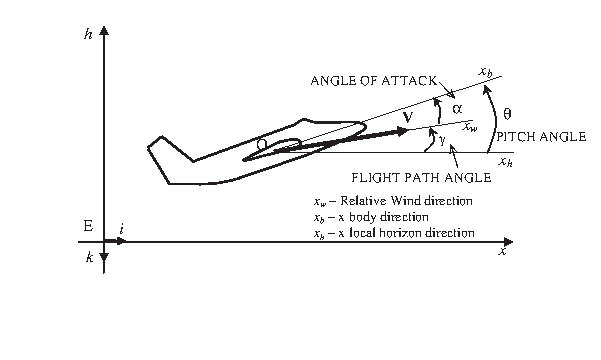
\includegraphics[width=1\textwidth]{AOA.png}
\caption{The angle of attack description for an aircraft in flight. [1]}
\label{fig:Figure1}
\end{figure}

\begin{figure}[here]
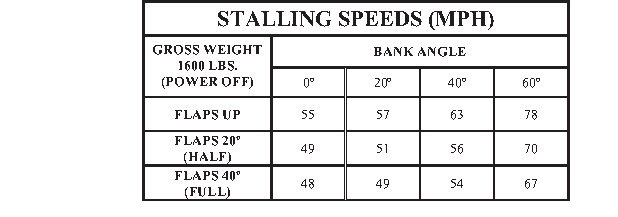
\includegraphics[width=0.9\textwidth]{stall_speed.png}
\caption{Given stall speeds for the CESSNA 150 at a weight of 1600 lbs. [1]}
\label{fig:Figure2}
\end{figure}


\end{document}